\section{Free selective functors}\label{sec-free}

The idea of describing effectful computations using \emph{free constructions},
such as \emph{free}~\cite{swierstra2008data} and \emph{freer
monads}~\cite{kiselyov2015freer} and \emph{free applicative
functors}~\cite{free-applicatives} is well-studied in the functional programming
community. Free constructions allow us to focus on the internal aspects of the
effect under consideration and receive the desired applicative or monadic
computation structure \emph{for free}, i.e. without the need to define custom
instances or prove laws.

In this section we apply this idea to selective functors. We present a free
construction for \emph{rigid} selective functors
(\S\ref{sec-free-construction}), and demonstrate it on two examples
in~\S\ref{sec-free-ping-pong} and~\S\ref{sec-free-isa}.

\subsection{Free construction}\label{sec-free-construction}

In the free structures methodology, the essence of an effect is captured by a
data type that encodes the ``commands'' which the effect provides, acting as a
deep embedding of the effect's interface. This data type needs only have enough
structure to be a~\hs{Functor}. The purpose of a free construction is then to
build a richer structure on top of this \emph{base functor}, which would have
the desired instances, in our case \hs{Applicative} and \hs{Selective}. In this
section we will denote the base functor by \hs{f}.

\begin{figure}
\begin{minted}[fontsize=\small]{haskell}
data Select f a where
    Pure   :: a -> Select f a
    Select :: Select f (Either a b) -> f (a -> b) -> Select f b
\end{minted}
\vspace{0mm}
\begin{minted}[fontsize=\small]{haskell}
instance Functor f => Functor (Select f) where
    fmap f (Pure a)     = Pure (f a)
    fmap f (Select x y) = Select (fmap f <$> x) (fmap f <$> y) -- Free theorem from Fig. 4
\end{minted}
\vspace{0mm}
\begin{minted}[fontsize=\small]{haskell}
instance Functor f => Applicative (Select f) where
    pure  = Pure
    (<*>) = apS -- Law of rigid selective functors
\end{minted}
\vspace{0mm}
\begin{minted}[fontsize=\small]{haskell}
instance Functor f => Selective (Select f) where
    select x (Pure y)     = either y id <$> x -- Generalised identity
    select x (Select y z) = Select (select (f <$> x) (g <$> y)) (h <$> z) -- Associativity
      where
        f x = Right <$> x
        g y = \a -> bimap (,a) ($a) y
        h z = uncurry z
\end{minted}
\vspace{0mm}
\begin{minted}[fontsize=\small]{haskell}
-- Lift a base functor into Select
liftSelect :: Functor f => f a -> Select f a
liftSelect f = Select (Pure (Left ())) (const <$> f)
\end{minted}
\vspace{0mm}
\begin{minted}[fontsize=\small]{haskell}
-- Interpret a free selective structure given a natural transformation from f to g
runSelect :: Selective g => (forall x. f x -> g x) -> Select f a -> g a
runSelect _ (Pure a)     = pure a
runSelect t (Select x y) = select (runSelect t x) (t y)
\end{minted}
\vspace{0mm}
\begin{minted}[fontsize=\small]{haskell}
-- Extract the resulting value from a pure selective computation
getPure :: Select f a -> Maybe a
getPure = runSelect (const Nothing)
\end{minted}
\vspace{0mm}
\begin{minted}[fontsize=\small]{haskell}
-- Extract all possible effects from a selective computation
getEffects :: Functor f => Select f a -> [f ()]
getEffects = getOver . runSelect (Over . pure . void)
\end{minted}
\vspace{-3mm}
\caption{Free rigid selective functors (various performance improvements
omitted for clarity).}\label{fig-free}
\vspace{-3mm}
\end{figure}

As we remarked in~\S\ref{sec-laws}, rigid selective functors have a particularly
simple normal form thanks to the additional law \hs{(<*>)}~\hs{=}~\hs{apS},
which tells us that the apply operator \hs{<*>} is redundant and can be
implemented via the selective interface. This normal form has the following
linear structure:

\vspace{1mm}
\begin{minted}[xleftmargin=10pt]{haskell}
pure x <*? fa <*? fb <*? ... <*? fy
  where
    x  :: Either a (Either b (Either c (... z)))
    fa :: f (a ->   Either b (Either c (... z)))
    fb :: f (b ->             Either c (... z))
    ...
    fy :: f (y ->                           z)
\end{minted}
\vspace{1mm}

\noindent
In words, any rigid selective computation can be rewritten as a left-associated
sequence of select operators, where the initial pure value~\hs{x} comes from a
large sum type (comprising alternatives~\hs{a} to~\hs{z} in the above snippet),
and each effect in the sequence of select operators eliminates one of the
alternatives, in order, until only one remains (namely, \hs{z}). Interestingly,
there is no right-associative version of the normal form, because the
associativity law can only be used to re-associate a given expression to the
left (\S\ref{sec-laws}). To apply it in reverse, we would need to ``factor out''
the reshaping functions \hs{f}, \hs{g} and \hs{h} from the base functor, which
is not always possble. This is different from applicative functors that have two
normal forms corresponding to left and right
re-association~\citep{free-applicatives}.

Fig.~\ref{fig-free} gives an encoding of this normal form in Haskell. The free
data type \hs{Select} has two constructors: \hs{Pure}, to embed pure values in
a selective computation, and \hs{Select} to build type-aligned sequences of
base functor effects, by appending new effects to the right end of the sequence.
The sequence can only be started with the \hs{Pure} constructor, thus enforcing
the normal form. Implementation of instances relies on the laws presented
in~\S\ref{sec-laws}: generalised identity, associativity, as well as one of the
free theorems. We do not need the distributivity law, since it is subsumed by
the law of rigid selective functors \hs{(<*>)}~\hs{=}~\hs{apS}, which is used
directly in the \hs{Applicative} instance.

Effects from the base functor can be embedded in the free construction using
the helper function \hs{liftSelect}. To interpret a free selective computation
\hs{Select}~\hs{f}~\hs{a} in a selective functor \hs{g}, one needs to provide
a \emph{natural transformation} from \hs{f} to \hs{g} to the function
\hs{runSelect}, which traverses the sequence of effects converting them to
\hs{g} and composing the results using \hs{g}'s select operator.

For example, \hs{getPure} reinterprets a given free computation in the selective
functor \hs{g}~\hs{=}~\hs{Maybe} using the natural transformation
\hs{const}~\hs{Nothing}, which leaves the \hs{Pure} head of the sequence as is,
but turns any subsequent effect into \hs{Nothing}. Similarly, \hs{getEffects}
records all effects by stashing them in the selective functor \hs{Over}, which
are subsequently extracted from it by \hs{getOver}.

We do not present a free construction for non-rigid selective functors here but
it can be found in the module \cmd{Control.Selective.Free} of the
library~\citep{selective2019haskell} and in the supplementary material.

\subsection{Ping-pong, freely}\label{sec-free-ping-pong}

To illustrate the usage of the free selective functors on a simple example,
we implement the classic \cmd{Teletype} DSL~\cite{swierstra2008data} comprising
two commands: \emph{reading} a string form the input stream and \emph{writing}
a string to the output stream. The base functor has two corresponding
constructors:

\vspace{1mm}
\begin{minted}[xleftmargin=10pt]{haskell}
data Teletype a = Read (String -> a) | Write String a deriving Functor
\end{minted}
\vspace{1mm}

\noindent
For convenience, we can provide the following functions that embed the commands
into the free selective construction, mimicking Haskell's \hs{IO} API:

\vspace{1mm}
\begin{minted}[xleftmargin=10pt]{haskell}
getLine :: Select Teletype String
getLine = liftSelect (Read id)
\end{minted}
\vspace{0mm}
\begin{minted}[xleftmargin=10pt]{haskell}
putStrLn :: String -> Select Teletype ()
putStrLn s = liftSelect (Write s ())
\end{minted}
\vspace{1mm}

\noindent
We can now reimplement the \hs{pingPongS} example from~\S\ref{sec-intro} in
terms of the free selective construction simply by adjusting the type signature.
Note that the \hs{whenS} combinator comes for free.

\vspace{1mm}
\begin{minted}[xleftmargin=10pt]{haskell}
pingPongS :: Select Teletype ()
pingPongS = whenS (fmap (=="ping") getLine) (putStrLn "pong")
\end{minted}
\vspace{1mm}

\noindent
By embedding \hs{pingPongS} into the free construction, we gain access to the
static analysis machinery:

\vspace{1mm}
\begin{minted}[xleftmargin=10pt]{haskell}
@\ghci@ getEffects pingPongS
[Read,Write "pong"]
\end{minted}
\vspace{1mm}

\noindent
The \hs{getEffects} function (Fig.~\ref{fig-free}) returns a list of all effects
of a free selective computation. In the case of the \hs{Teletype} functor, we
get a list of all commands that a computation might execute.

We can interpret \cmd{Teletype} programs in any other selective functor using
the \hs{runSelect} function by providing a natural transformation
\hs{forall}~\hs{x.}~\hs{Teletype}~\hs{x}~\hs{->}~\hs{g}~\hs{x}, which assigns an
interpretation to \cmd{Teletype} commands in terms of \hs{g}. A good example of
such transformation would be an interpretation in the \hs{IO} monad, which
allows us to execute our \hs{pingPongS} program:

\vspace{1mm}
\begin{minted}[xleftmargin=10pt]{haskell}
toIO :: Teletype a -> IO a
toIO (Read f)    = f <$> Prelude.getLine
toIO (Write s a) = a <$  Prelude.putStrLn s
\end{minted}
\vspace{0mm}
\begin{minted}[xleftmargin=10pt]{haskell}
@\ghci@ runSelect toIO pingPongS
hello
@\ghci@ runSelect toIO pingPongS
ping
pong
\end{minted}
\vspace{1mm}

\noindent
Note that while we can write simple programs like \hs{pingPongS} using the
selective interface, we are fundamentally limited in what we can express
compared to the much more powerful monadic interface. As an example, consider
this simple greeting program:

\vspace{1mm}
\begin{minted}[xleftmargin=10pt]{haskell}
greeting = getLine >>= \name -> putStrLn ("Hello " ++ name)
\end{minted}
\vspace{1mm}

\noindent
Programs like this cannot be expressed in our simple \cmd{Teletype} DSL. Even if
we had \hs{bindS} for strings~(\S\ref{sec-alt-multi}), it would be useless for
static analysis because it would have to report effects \hs{Write}~\hs{s} for
\emph{all possible strings} \hs{s}! Nevertheless, limitations of the selective
interface can sometimes be worked around by using more sophisticated base
functors, as we show in~\S\ref{sec-free-isa}.

% Software build systems can be modelled with purely functional
% abstractions~\cite{mokhov2018build} that enable the model to accommodate many
% different build systems and express their features in a way that allow for deriving
% new build systems by combining the best parts of the existing ones. The approach
% presented on~\cite{mokhov2018build} allows to distinguish the \emph{static} build
% dependencies from the \emph{dynamic} ones by expressing the build tasks which
% may only have static dependencies with the \hs{Applicative} interface, and using
% \hs{Monad} for constructing build tasks with dynamic dependencies.
% As selective functors give us the best of both worlds, we show how we could adopt
% their free construction to build a deep embedding of the \hs{fetch} callback from
% the original paper.

% To use any free construction, we need to invent an underlying functor, which would
% be the essence of the effect we are trying to implement. In case of the \hs{fetch}
% callback, we require an effect of a read-only store:

% \begin{minted}[xleftmargin=10pt]{haskell}
% data Fetch k v a = Fetch k (v -> a)
%    deriving Functor
% \end{minted}

% That is, the \hs{Fetch} functor has only one data constructor, which represents a
% command with a suggested semantics of extracting a value associated with a key from
% the store.

% We cannot directly use the \hs{Fetch} command in a selective computations, thus we
% embed it into a free selective construction by simply lifting the data constructor
% in the following way:

% \begin{minted}[xleftmargin=10pt]{haskell}
% fetch :: k -> Select (F k v) v
% fetch key = liftSelect $ Fetch key id
% \end{minted}

\subsection{Analysis and simulation of processor instructions}\label{sec-free-isa}

To demonstrate the free construction on a more interesting example, we apply it
to analysis and simulation of a hypothetical instruction set architecture
(ISA)\footnote{Incidentally, this was the original motivation for selective
functors. While describing the formal semantics of instructions of a real
processor, we needed a statically analysable \hs{ifS} for the purpose of
symbolic program verification, which eventually led us to \hs{select}. We use a
hypothetical ISA in this section instead of the real one, because of the
complexity of the latter.}. By expressing the ISA semantics in our
free construction with an unusual base functor, we will be able to build
tools both for static data flow analysis and simulation of programs with
branching.

\subsubsection{ISA semantics}

To work around some of the aforementioned limitations of the selective
interface (namely, the lack of the bind operator), we represent the semantics of
instructions thus:

\vspace{1mm}
\begin{minted}[xleftmargin=10pt]{haskell}
type Program a = Select RW a
\end{minted}
\vspace{0mm}
\begin{minted}[xleftmargin=10pt]{haskell}
data RW a = Read  Key                 (Value -> a)
          | Write Key (Program Value) (Value -> a) deriving Functor
\end{minted}
\vspace{1mm}

\noindent
The \hs{RW} (pronounced ``read-write'') base functor encodes the effect of a
mutable key-value store comprising two commands: (i)~we need the ability to
\emph{read} a value associated with a key from the store, and (ii) given a
computation which produces a value, \emph{write} its result into the store.
Think of \hs{Value} as a machine word, and \hs{Key} as an ISA memory location
(a register, a memory cell, or a processor flag). The base commands are similar
to \cmd{Teletype}, with one key difference: the \hs{Write} constructor takes
\hs{Program}~\hs{Value}, i.e. a computation producing a value instead of just
plain \hs{Value}.

This exact structure of the definition is required for accommodating a pattern
that occurs frequently in instruction semantics: often we read a value from a
register or a memory cell, do something with it, and then write it somewhere
else. If \hs{Write} required the second argument to be a pure value, as in
\cmd{Teletype}, we would not be able to express the desired pattern without
resorting to the monadic interface. Additionally, we want the \hs{Write}
command to not just write the value and return \hs{()}, but to \emph{give the
just written value back}, so it can be used in the rest of the computation; such
generosity of the \hs{Write} command will be useful for avoiding duplicating
data dependencies.

We introduce two convenience combinators, which lift the data constructors of
the \hs{RW} data type into the free selective, thus making them directly usable
in the definitions of instruction semantics:

\vspace{1mm}
\begin{minted}[xleftmargin=10pt]{haskell}
read :: Key -> Program Value
read k = liftSelect (Read k id)
\end{minted}
\vspace{0mm}
\begin{minted}[xleftmargin=10pt]{haskell}
write :: Key -> Program Value -> Program Value
write k fv = liftSelect (Write k fv id)
\end{minted}
\vspace{1mm}

\subsubsection{Example 1. Addition}

To get acquainted with the introduced vocabulary, we start by describing the
semantics for the addition instruction, which reads the summands from a
register and a memory cell, adds them, writes the result back into the same
register, and also updates the state of the \hs{Zero} flag to indicate whether
the resulting value is zero.

\begin{minted}[xleftmargin=10pt]{haskell}
add :: Register -> Address -> Program Value
add reg addr = let arg1     = read (Reg reg)
                   arg2     = read (Cell addr)
                   result   = (+)   <$> arg1 <*> arg2
                   isZero   = (==0) <$> write (Reg reg) result
               in write (Flag Zero) (bool 0 1 <$> isZero)
\end{minted}
\vspace{1mm}

\noindent
Here, we \hs{read} the summands \hs{arg1} and \hs{arg2} from the two specified
locations and calculate the \hs{result} of addition by lifting \hs{(+)} into the
free selective functor using applicative combinators. We then calculate the
value of the \hs{Zero} flag in a similar way, but here we exploit the fact that
the \hs{write} combinator returns the value it has just written, thus we can
reuse the \hs{result} without recalculating it from scratch.

By analysing the free semantics of the \hs{add} instruction, we can obtain the
list of all its effects, in the order they appear in the computation. We also
visualise the effects as a data flow graph, where data locations are shown as
rectangles, instructions as rounded rectangles, and reads/writes as arcs.

% \footnote{For didactic purposes,
% these graph was hand-crafted, but it is possible to get similar results
% automatically with Graphviz~\cite{ellson2001graphviz}.}

\vspace{-1mm}
\begin{figure}[!h]
\begin{minipage}{0.53\textwidth}
\raggedleft
\begin{minted}[xleftmargin=10pt]{haskell}
@\ghci@ getProgramEffects (add R0 1)
[Read R0,Read 1,Write R0,Write Zero]
\end{minted}
 \end{minipage}
 \begin{minipage}{0.44\textwidth}
  \centering
  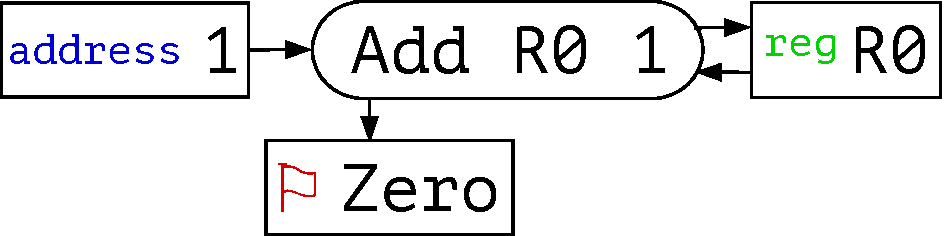
\includegraphics[scale=0.3]{fig/add.pdf}
 \end{minipage}
\end{figure}
\vspace{-1mm}

\noindent
To implement \hs{getProgramEffects}, we apply the natural transformation
\hs{toOver} to the effects of a \hs{Program}, which recursively collects the
effects that occur in the \hs{Write}'s argument \hs{fv}:

\vspace{1mm}
\begin{minted}[xleftmargin=10pt]{haskell}
getProgramEffects :: Program a -> [RW ()]
getProgramEffects = getOver . runSelect toOver
\end{minted}
\vspace{1mm}
\begin{minted}[xleftmargin=10pt]{haskell}
toOver :: RW a -> Over [RW ()] a
toOver (Read  k _   ) = Over [Read k (const ())]
toOver (Write k fv _) = runSelect toOver fv *> Over [Write k fv (const ())]
\end{minted}
\vspace{1mm}

\noindent
The semantics of the addition instruction has only used applicative combinators
and we thus could have analysed it statically using free applicative functors.
However, there are important instructions whose semantics cannot be expressed
in terms of the \hs{Applicative} interface, and this is where the presented
free selective construction becomes irreplaceable.

\subsubsection{Example 2. Conditional jump}

Selective functors introduce limited dependencies between effectful
computations, giving us enough power to express the semantics of branching
instructions, which modify the program counter by a given offset if a certain
condition holds. Consider the following instruction that performs a jump if the
result of the previous operation was zero.

\vspace{1mm}
\begin{minted}[xleftmargin=10pt]{haskell}
jumpZero :: Value -> Program ()
jumpZero offset = let zeroSet  = (==1) <$> read (Flag Zero)
                      modifyPC = void $ write PC ((+offset) <$> read PC)
                  in whenS zeroSet modifyPC
\end{minted}
\vspace{1mm}

\noindent
Here we use the \hs{whenS} combinator to modify the program counter only if
the \hs{Zero} flag is set. By implementing \hs{jumpZero} in terms of the
selective interface, we achieve both the ability to implement an adequate
simulator for branching programs and perform their static analysis:

\begin{figure}[!h]
 \begin{minipage}{0.45\textwidth}
\raggedleft
\begin{minted}[xleftmargin=7pt]{haskell}
@\ghci@ getProgramEffects (jumpZero 42)
[Read Zero,Read PC,Write PC]
\end{minted}
 \end{minipage}
 \begin{minipage}{0.54\textwidth}
  \centering
  
\includegraphics[scale=0.3]{fig/jumpZero.pdf}
 \end{minipage}
\end{figure}

\noindent
Since the analysis is static, the resulting list of effects and the
corresponding data flow graph are over-approximated and show all effects that
can possibly happen in the computation.

% Note that it does not matter which argument we supply to \hs{jumpZero}, since
% it will never get forced, e.g. the analysis will succeed and give us the same
% result even if we supply \hs{undefined}.

\subsubsection{Blocks of instructions}

Once we have implemented the semantics for a desired subset of an ISA, we can
describe the semantics of sequences, or \emph{blocks}, of instructions by
simply composing the semantics of individual instructions using the applicative
sequencing operator (\hs{*>}):

\vspace{1mm}
\begin{minted}[xleftmargin=10pt]{haskell}
addAndJump :: Program ()
addAndJump = add R0 1 *> jumpZero 42
\end{minted}
\vspace{1mm}

\noindent
We can analyse such compound computations in the same way as we analyse
individual instructions:

\vspace{-1mm}
\begin{figure}[!h]
 \begin{minipage}{0.46\textwidth}
\raggedleft
\begin{minted}{haskell}
@\ghci@ getProgramEffects addAndJump
[Read R0,Read 1,Write R0,Write Zero
,Read Zero,Read PC,Write PC]
\end{minted}
 \end{minipage}
 \begin{minipage}{0.50\textwidth}
  \centering
  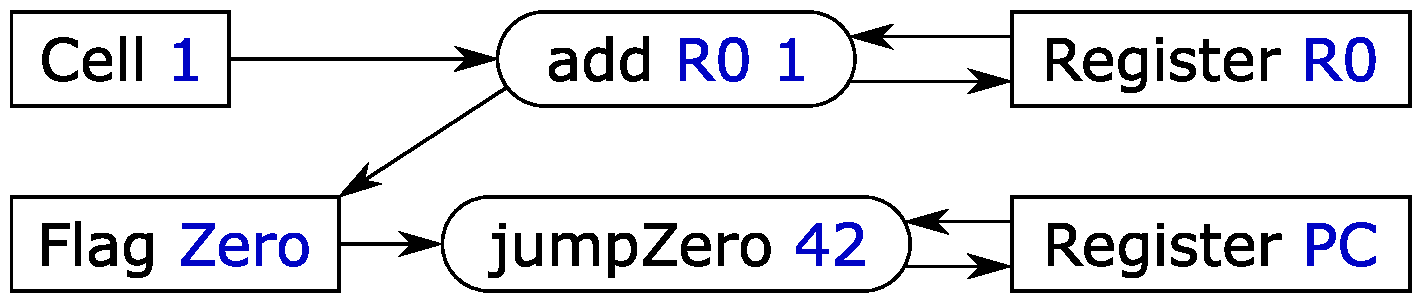
\includegraphics[scale=0.3]{fig/addAndJump.pdf}
 \end{minipage}
\end{figure}
\vspace{-1mm}

% Getting a flat list of effects that blocks of code perform is not very useful,
% since they does not carry any explicit data-flow information. To mitigate this
% restriction, we take the following approach. We create a (1) deeply-embedded
% assembly language and (2) implement an interpreter which assigns a semantics to
% this language in terms of the free selective construction. By doing this, we can
% then implement a mechanical procedure which would construct \emph{data flow
% graphs} of sequences of instructions, similar to the ones shown in
% Fig.~\ref{fig-addAndJump-gcd} by overlaying the graphs for single instructions.
% Note that if an instruction performs multiple read/writes of the same location,
% we will deliberately merge them in the resulting graph.

\subsubsection{Simulation}

To implement an ISA simulator, we follow the same path as in the \hs{pingPongS}
example and the \hs{IO} monad earlier in~\S\ref{sec-free-ping-pong}. We need a
natural transformation from the base functor \hs{RW} to an appropriate target
functor, e.g. an instance of \hs{MonadState}~\hs{ISAState}, where \hs{ISAState}
represents the state of all registers, memory cells and flags. For brevity, we
present only one part of such a transformation, which assigns an interpretation
to reading and writing of register keys~\hs{Reg}:

\vspace{1mm}
\begin{minted}[xleftmargin=10pt]{haskell}
toState :: MonadState ISAState m => RW a -> m a
toState (Read k t) = t <$> case k of
    Reg r -> (Map.! r) <$> gets registers -- Look up r in the registers field
    ...
toState (Write k fv t) = case k of
    Reg r -> do v <- runSelect toState fv -- Evaluate the Write's argument first
                let step s = Map.insert r v (registers s)
                state $ \s -> (t v, s { registers = step s })
    ...
\end{minted}
\vspace{1mm}

\noindent
To read a register, we simply lift the lookup function \hs{Map.!} to the
corresponding field of the \hs{ISAState}. To write an effectful value \hs{fv}
into a register, we need to evaluate it first; hence we call the \hs{runSelect}
function, supplying it the natural transformation \hs{toState}, recursively,
thus performing the effects of \hs{fv}. We then adjust the register bank with
the new value and return it.

The natural transformation \hs{toState} gives interpretation to individual
\hs{Read} and \hs{Write} commands, and now this interpretation can be extended
to any \hs{Program} by plugging it into a \hs{runSelect} call, as has already
been done once in the implementation of \hs{toState} itself:

\vspace{1mm}
\begin{minted}[xleftmargin=10pt]{haskell}
runProgram :: Program a -> ISAState -> (a, ISAState)
runProgram p = runState (runSelect toState p)
\end{minted}

\subsubsection{Restrictions}

The free selective construction in combination with the base functor \hs{RW}
provides an abstraction capable of expressing the semantics of arithmetic,
load/store and branching instructions. However, one should remember that
selective functors still lack the full expressive power of the monadic interface
and are unable to accommodate an important class of instructions, specifically
those that use the \emph{memory-indirect addressing mode}. If we had a
\hs{Monad}~\hs{Program} instance, we could give the following semantics to the
memory-indirect load instruction \hs{loadMI}:

\vspace{1mm}
\begin{minted}[xleftmargin=10pt]{haskell}
loadMI :: Register -> Address -> Program Value
loadMI reg addr = read (Cell addr) >>= \x -> write (Reg reg) (read (Cell x))
\end{minted}
\vspace{1mm}

\noindent
Here, we read from a memory cell \hs{addr}, then use the monadic bind operator
to extract a value~\hs{x} from the result, and use it in a subsequent memory
read \emph{as address}. Although this semantics is, in principle, implementable
using the selective \hs{bindS} combinator (see \S\ref{sec-alt-multi}), it is not
very useful in practice since static analysis would record possible access to
\emph{all memory cells}~\hs{x}, and there are too many of them (typically, a
large power of two). Furthermore, the execution of the resulting semantics would
be terribly slow, since it would also follow the same linear exploration of the
memory address space (although see \S\ref{sec-alt-multi} for a possible solution
of the performance issue).

% not get any strong benefits. Specifically, since the \hs{getProgramEffects} function,
% which performs static analysis of effects, constructs a conservative
% over-approximation, it would always report something similar to this:
% \hs{[Read addr,Write reg, Write reg...}, which would contain as much instances
% of the \hs{Write} effects as much inhabitants there are in the address
% datatype (usually a large power of two).  Therefore, we lose static analysis.
% Maybe we could get some benefit in simulation? No, unfortunately we, again,
% will not, since \hs{bindS} cannot get magically translated to the monadic
% \hs{>>=}, but instead performs explicit enumeration of inhabitants of the
% bound variable's type, which causes terrible performance regression comparing
% to a monadic implementation. Considering these arguments, using \hs{bindS} for
% mimicking monadic behaviour is not feasible in our case and memory-indirect
% load cannot be modelled in by means of the \hs{ISA} datatype.
